\section{Implementation}
    The following section largely documents the system as it was developed
    chronologically, and is not representative of the order in which systems are
    initialised in the final piece of software. This better highlights the
    dependencies between each discrete stage in development and reinforces the
    plan-driven approach to the project as a whole.

\subsection{System initialisation}
    There are two main files which handle the entirety of system startup, namely
    \code{linker.ld} and \code{boot.S}, the former responsible for defining the
    layout of the final executable we will be producing, and the latter handling
    the setup of the C runtime environment and passing control to the main
    kernel function.

    \subsubsection{Linker Script}
        \label{sec:Linker}
        In order to create a kernel, or any program for that matter, we must
        link all compiled object files into a single executable. For user-space
        programs, that is, programs written to run in an established operating
        system, there are default scripts provided by the compiler which do
        this. Since the operating system on which we will run the kernel does
        not yet exist, we must create a linker script ourselves.

        We begin by declaring that the symbol \code{\_start} is the entry point
        for our entire program (this is usually \code{main} for user-space
        programs), meaning execution will jump to this address when the system
        starts. We first declare the symbols \code{\_\_start} and
        \code{\_\_text\_start} at address \code{0x8000}, which informs the
        bootloader where to place our kernel image. Addresses up to
        \code{0x8000} will be reserved for the stack. After this we must declare
        one by one each of the major sections which will be used in the ELF
        file, the first of which is the \code{.text} section, containing
        executable code.  The code from \code{boot.S} is placed in the
        \code{.text.boot} section, and we use the \code{KEEP} directive to
        inform the linker not to optimise the code in that section -- we want it
        running exactly what is written there. We declare the sections
        \code{.rodata}, \code{.data}, and \code{.bss} similarly, each time
        declaring global symbols for them should the need to use them as
        variables arise (as is the case, for example, when placing the metadata
        for pages directly after the kernel image, see Section \ref{sec:pages}).
        We also use the directive \code{ALIGN} to define a page size for the
        kernel image -- specifically, this sets the current address to the next
        available address that is divisible by the page size we set, 4096 bytes.

    \subsubsection{Initialising the C runtime}
        With our kernel image sections defined, we can actually write the code
        that will boot into our kernel, contained in the file \code{boot.S}. We
        begin by declaring that this is to be placed in the \code{.text.boot}
        section (as used by the bootloader) and we make our start symbol visible
        from any file using the \code{.global} directive -- this is required for
        the linker to see which location to jump to at system startup.

        The project was initially written for the Raspberry Pi 2, containing the
        quad-core Cortex-A7 CPU. However, since multicore programming entails
        extra difficulty even in a familiar user-space environment, it was
        always designed to only use one of these cores. The following code
        remains included in the project, wrapped in a test to determine which
        processor we have compiled for, and sends three of the four cores to
        hang. We will discuss it now to introduce the idea of the ARM
        coprocessor:

        \lstset{style=asm}
        \begin{lstlisting}[caption={Code to halt three of the four cores},captionpos=b]
_start:
    mrc p15, #0, r1, c0, c0, #5
    and r1, r1, #3
    cmp r1, #0
    bne halt
        \end{lstlisting}

        The \code{mrc} and \code{mcr} instructions allows for interaction with
        the system control processor, and denote ``move data from coprocessor to
        ARM register'' and ``move data from ARM register to coprocessor''
        respectively. The purpose of this is to control and provide status
        information for the functions implemented on the ARM1176JZF-S processor
        \cite[pg.~3-2]{TRM}, and exposes optional\footnote{ARM only provides
        specifications for processors; it is down to hardware manufacturers to
        implement their designs.} additional functionality that is not provided
        by the core instruction set. Among others, these functions include:
        \begin{itemize}
            \itemsep0em
            \item System control and configuration
            \item MMU control and configuration
            \item Cache control and configuration
            \item Direct Memory Access (DMA) control
            \item System performance monitoring
        \end{itemize}

        As it stands, the project only makes use of the first two functions. The
        code block itself reads the Multiprocessor Affinity Register
        \cite{MPIDR} for the identifier of the current CPU it is testing, and if
        neither of the two lower bits returned are 1, then the core is sent to
        halt indefinitely in a low-power state. Using the system control
        processor is simply a case of finding the desired functionality from
        \cite[pg.~3-14]{TRM} and copying the \code{mrc} or \code{mcr}
        instruction it specifies.

        With just a single core to develop for, the next step is to set up the
        stack pointer at address \code{0x8000}. The program counter for the
        kernel starts at address \code{0x8000} and grows upwards, and, since the
        stack grows downwards, it is safe to place it at this address without it
        interfering with the kernel. Next the start and end of the Basic Service
        Set (BSS) is loaded into registers -- recall that this is where
        statically allocated global variables are stored. Since the C standard
        requires uninitialised global variables to be zeroed, we must zero out
        (that is, store the value 0) in the registers between the addresses of
        \code{\_\_bss\_start} and \code{\_\_bss\_end}.

        The final responsibility of \code{boot.S} is to transfer control to our
        kernel entry point, \code{kernel\_main}, by loading the address of this
        symbol into the program counter. Overall, this small portion of the
        codebase initialises a minimum C environment, meaning the stack is
        initialised and the BSS segment zeroed before we pass control to our
        custom kernel. Note that the use of registers 0, 1, and 2 is avoided as
        the bootloader uses these to pass system parameters and hardware
        information to the main function\footnote{Namely, the device from which
        the system was booted, the ARM Linux Machine Type (\code{0xc42} for the
        Pi), and the address of the atags, which contain more important
        information such as available memory.} at runtime.

\subsection{Organising memory}
    \subsubsection{Atags}
        One important piece of data passed by the bootloader to the main kernel
        function is the address of the ``atags'' -- this is a list of tags which
        describe various system parameters such as total system memory, the
        initial ramdisk, and command-line parameters to pass, and is passed
        through address \code{0x100} on the Raspberry Pi 1. Throughout the
        execution of the operating system, computations will require memory and
        since the project functions entirely in kernel-space, any and all memory
        is available to use. To impose some structure on the memory and manage
        it effectively, however, we organise it into 4kiB pages, allowing for
        equal-sized blocks of memory, which are neither insignificantly nor
        prohibitively large, to be allocated and tracked. Therefore, the most
        important piece of information among the atags is the total system
        memory, which the project uses in its implementation of a dynamic memory
        allocator.

        In order to parse this list of tags, we need the kernel to understand
        the layout of the data it is being passed. In particular, each tag
        consists of two values: an unsigned 32-bit integer denoting the length
        of the tag (in 32-bit words), and the tag itself, details of which are
        found at \cite{atags}. This provides information concerning the memory
        tag itself, namely that it contains two unsigned 32-bit integers
        describing memory size and start address, in this order. Therefore, we
        define the C structure \code{atag\_mem} to easily access these two
        fields once we come across the memory tag. Thus, to determine the total
        memory available we iterate over the atags list until we find the memory
        tag, cast this to our \code{atag\_mem} structure, and consequently
        return the field denoting the size of system memory.

    \subsubsection{Pages}
        \label{sec:pages}
        The total number of pages is the total size of memory divided by the
        page size, which we have set to 4kiB. In order to effectively manage
        each page, we create a list containing metadata for each page: this
        metadata includes, for example, the virtual address to which it maps,
        along with bit-field flags detailing whether the page is allocated, if
        it available for sharing, if it is a kernel page (for when user-space is
        implemented), and whether it is a regular page or a page on the heap.
        We use the global symbol \code{\_\_end}, declared in the linker script,
        to place the page metadata list directly after the end of the kernel
        image.

        To allocate a page, we need of knowledge of which ones are free to do
        so, for which we create a linked list of all such pages. Then all that
        is needed is to return a pointer to its location in memory and zero it
        (for security), modify the appropriate flags in the page array, and
        remove it from our free pages list. When a page's use is no longer
        required, it makes sense to make it available for future allocations,
        for example when a process has finished executing (see Section
        \ref{sec:cleanup}). Thus, to free a page we use its physical address to
        index into the array containing all pages, set the \code{allocated} to
        0, and add it back to the list of free pages.

    \subsubsection{Dynamic memory allocator}
        To allocate memory dynamically, and less restrictively than entire pages
        at a time, we reserve a 1MiB portion of memory directly after the page
        metadata for heap memory, which is used to allocate segments of memory
        instead, with a similar interface to the C standard library's
        \code{malloc} and \code{free}. This choice of 1MiB is fairly arbitrary,
        but is not too restrictive for most uses of dynamic memory and does not
        use too large a portion of memory that will eventually be used by
        user-space.
        
        Memory allocation is implemented by first defining for each allocation a
        header containing the allocation size, in bytes, and whether it has been
        allocated, and then using these headers to form a linked list. Thus, in
        order to grant an allocation we must find a header that is at least the
        requested number of bytes in size, and not currently in use. If the
        best-fitting segment, that is, the segment with the smallest size that
        satisfies the request, is relatively large compared to what was
        requested, we split it so that we may use what is effectively ``left
        over'' to satisfy some future request.

        When freeing memory allocations, we mark the segment as unallocated by
        modifying the bit in the allocation header and merge adjacent free
        segments in the linked list into one, thus decreasing the likelihood of
        internal fragmentation -- unused or unusable memory within the segment
        \cite[pg.~363]{DinosaurOS}. Coalescing adjacent free segments to the
        left is shown below; the process is identical for coalescing to the
        right, except that it modifies the pointer to the \code{next} segment
        header instead.
        \lstset{language=c}
        \begin{lstlisting}[caption={Coalescing heap segments to the left},captionpos=b]
/* merge segments to the left */
while (seg->prev != NULL && !seg->prev->allocated) {
    seg->prev->next = seg->next;
    seg->prev->segment_size += seg->segment_size;
    seg = seg->prev;
}
        \end{lstlisting}

        When initialising the heap at system startup, we must first allocate the
        appropriate number of pages and mark them as kernel heap pages, then
        initialise the linked list of segments by declaring a single segment
        1MiB in size. Although the total heap size remains the same, it will
        become split into increasingly many segments, all forming a linked list,
        as allocation requests are satisfied.

\subsection{Serial Output}
    \label{sec:GPIO}
    An operating system would be useless without an efficient means of
    interacting with it during execution, so the next task to present itself was
    that of interfacing with the Universal Asynchronous Receiver/Transmitter, a
    peripheral on the Pi, which is capable of serial\footnote{One bit at a time}
    communication. While output would evolve to be via HDMI, it was simpler to
    initialise this when working within QEMU, and also prompted for an intuitive
    interface for GPIO to be written, which would again become useful when
    debugging with HDMI output.

    \subsubsection{Peripherals}
        As mentioned, a peripheral is a device with a specific address from and
        to which it may read and write data, and all interactions with
        peripherals make use of Memory Mapped I/O (MMIO) to do so on the
        Raspberry Pi -- the process of performing I/O by reading from and
        writing to predefined memory address. Moreover, each peripheral may be
        described by an offset from the Raspberry Pi's Peripheral Base Address.
        This varies for different models of the Pi, but on the Raspberry Pi 1
        Model B+, this is located at address \code{0x20000000}, and the physical
        address for peripherals span from this base address up to
        \code{0x20ffffff}. The peripheral itself contains a collection of
        registers which may be read and written, and these are defined at
        offsets from that specific peripheral's base address (see Table
        \ref{tab:UART} for clarification).

        \begin{table}
            \centering
            \begin{tabular}{|c|l|c|}
                \hline
                \textbf{Offset} & \textbf{Register} & \textbf{Size} \\
                \hline
                \code{0x00} & Data Register & 32 \\ \hline
                \code{0x04} & RSRECR & 32 \\ \hline
                \code{0x18} & Flag Register & 32 \\ \hline
                \code{0x20} & Unused & 32 \\ \hline
                \code{0x24} & Integer Baud Rate Divisor & 32 \\ \hline
                \code{0x28} & Fractional Baud Rate Divisor & 32 \\ \hline
                \code{0x2c} & Line Control Register & 32 \\ \hline
                \code{0x30} & Control Register & 32 \\ \hline
                \code{0x34} & Interrupt FIFO Level Select Register & 32 \\ \hline
                \code{0x38} & Interrupt Mask Set Clear Register & 32 \\ \hline
                \code{0x3c} & Raw Interrupt Status Register & 32 \\ \hline
                \code{0x40} & Masked Interrupt Status Register & 32 \\ \hline
                \code{0x44} & Interrupt Clear Register & 32 \\ \hline
                \code{0x48} & DMA Control Register & 32 \\ \hline
                \code{0x80} & Test Control Register & 32 \\ \hline
                \code{0x84} & Integration Test Input Register & 32 \\ \hline
                \code{0x88} & Integration Test Output Register & 32 \\ \hline
                \code{0x8c} & Test Data Register & 32 \\ \hline
            \end{tabular}

            \caption{Each register is described by an offset from the UART base
            address, \code{0x20201000}.}
            \label{tab:UART}
        \end{table}

        There are several steps to initialise the UART for use on the Pi, and
        involves setting various configuration flags. The following steps are
        performed in order in \code{uart\_init()} in \code{gpio.c}:
        \begin{enumerate}
            \itemsep0em
            \item disable all aspects of the UART
            \item disable all GPIO pins
            \item disable pins 14 and 15
            \item clear all pending interrupts
            \item set up the baud rate of the connection
            \item enable FIFOs and set word length to 8 bits
            \item disable all interrupts
            \item enable the UART hardware, and the ability to transmit and
                receive data
        \end{enumerate}

        To send a byte to the data register, we wait until the FIFO (the data
        structure by which the UART sends and stores information) is not full
        and write the byte to the data register. Receiving a byte is done by
        waiting until the FIFO is non-empty and returns whatever is in the data
        register. Thus we have serial input and output, and may use this to
        implement \code{putc} and \code{getc} respectively. When running this
        build on QEMU, passing the \code{-serial} flag enables the sending and
        receiving of serial output via the host computer, thus we can specify
        \code{stdin} to be able to send character input via the host system's
        keyboard. This enables us complete interactivity with the kernel in the
        emulated environment.

\subsection{Interacting with the GPU}
    While QEMU was a powerful tool to allow for quick development and
    testing of core low-level features, as discussed its lack of simulation
    of a system timer required that the project eventually be moved to real
    hardware to tackle core features such as processes and interrupts.
    Furthermore, the Pi comes without a dedicated serial port, therefore without
    a TTL-to-USB adapter we are unable to use the UART to output to a real
    screen. Instead, it is much more natural to use the onboard HDMI port to
    output to a display, and for this we require communicating with the GPU.

    Displaying anything to the screen via the HDMI requires the use of a
    framebuffer; this is a piece of memory which is shared between the CPU and
    GPU. The CPU writes RGB pixels to the buffer and the GPU reads from it to
    render the pixels to whichever output device is connected. We must first
    request a framebuffer from the GPU, and this interaction takes place over
    the mailbox peripheral.

    \subsubsection{Mailbox Peripheral}
        The mailbox peripheral is a peripheral, just like the UART, which
        facilitates communication between the CPU and GPU, more specifically the
        VideoCore Operating System, and starts at offset \code{0xb880}
        \cite{Mailboxes}. It contains a read register, located at offset
        \code{0x0} from the base, which holds messages sent by the GPU; a status
        register, located at offset \code{0x18}, which is used to signify
        whether the read register is empty or full; and a write register,
        located at offset \code{0x20}, which the CPU can use to send data to the
        GPU. Since the mailbox peripheral can also be used to send and receive
        information about multiple systems, such as power management, audio, and
        the on-board camera, the peripheral requires communication through
        certain channels. This is simply a number that specifies the meaning
        behind the data being sent; for the framebuffer, we communicate via
        channel 1.

        Crucially, the process of communicating with the GPU via the mailbox
        peripheral differs depending on the model of Raspberry Pi being used;
        since the project was initially intended to run on the Pi 2 Model B, an
        interface was written for this version, however since it is a much
        simpler process on the Pi 1 Model B+, after some weeks debugging and
        making little progress, the decision to switch the target platform was
        switched at this point. Within the source code are both methods,
        and both are guarded by macros (see Section \ref{sec:directives} on
        Makefile directives) which will prevent compilation of the wrong one.

    \subsubsection{Initialising the framebuffer}
        We therefore require two functions to initialise the framebuffer: one to
        send the framebuffer request to the GPU, and one to read its response.
        These are implemented as \code{mailbox\_send()} and
        \code{mailbox\_read()} respectively. Both require as an argument the
        channel number through which to communicate, and the former requires the
        additional parameter of what to send. Since we are requesting a
        framebuffer, we map one out in a C structure containing all the fields
        necessary to fully describe this area of memory, such width, height, and
        the maximum number of columns and rows (for text). Listing
        \ref{lst:framebuffer} shows the entire structure used to describe the
        framebuffer in the operating system. Two important pieces of information
        we must set are the depth and the pitch of the framebuffer. The
        framebuffer's depth is the number of bits in every pixel; we are using 8
        bits for each of the red, green, and blue component, giving a total
        depth of 24. The pitch is the number of bytes per row of the screen. We
        can then calculate the number of pixels per row as $n = p *
        \frac{8}{d}$, where $p$ and $d$ are the values for pitch and depth,
        respectively. To calculate memory address $a$ of a pixel located at
        coordinate $(x,y)$ we have $a = p * y + (\frac{d}{8}) x$. To initialise
        the framebuffer, we define the values we wish to set in a temporary
        structure representing the request, send this request to the GPU through
        the mailbox via the framebuffer channel, and, if successful, write these
        values to the framebuffer.

        \lstset{language=c}
        \begin{lstlisting}[caption={Structure representing the
        framebuffer},captionpos=b,label={lst:framebuffer}]
struct framebuffer {
    uint32_t width;
    uint32_t height;
    uint32_t pitch;
    void    *buffer;
    uint32_t bufsize;
    uint32_t max_col;
    uint32_t max_row;
    uint32_t col;
    uint32_t row;
};
        \end{lstlisting}

    \subsubsection{Writing to the screen}
        The field \code{buffer} in the \code{struct framebuffer} is the area of
        memory to which we may write in order to display information on the
        screen, and in particular contains writing to it directly modifies the
        pixels displayed. Using the previous formula to determine the correct
        memory address to write for a given pixel, we implement this
        functionality as follows:

        \lstset{language=c}
        \begin{lstlisting}[caption={Implementation of \code{write\_pixel}},captionpos=b]
void write_pixel(uint32_t x, uint32_t y, const struct pixel *color) {
    uint8_t *loc = fb_info.buffer + y * fb_info.pitch + x * BYTES_PER_PIXEL;
    memcpy(loc, color, BYTES_PER_PIXEL);
}
        \end{lstlisting}

        This uses our own implementation of the C standard library's
        \code{memcpy} along with another structure \code{struct pixel}, which is
        simply three 8-bit unsigned integers describing the pixel's red, green,
        and blue values. For illustration, when the framebuffer is initialised
        we wish to clear the screen by writing black pixels to each location,
        resulting in 307,200 calls to \code{write\_pixel()} for a $640\times480$
        screen.

        With the ability to write arbitrary pixels on the screen, we
        may define a now define a font in order to write each individual pixel
        constituting a character, printing a character to the screen. For this
        purpose we use Daniel Hepper's $8\times8$ bitmap font \cite{DHepper},
        which simply defines for each character the pixels which are filled and
        unfilled. We also take inspiration from his rendering function, allowing
        us to determine whether the $n^{th}$ pixel is filled by right-shifting
        by $n$, using \code{write\_pixel()} in any case to modify the current
        pixel accordingly.

        In the function \code{gpu\_putc()}, we use this method to print only the
        printable ASCII characters (characters whose code is between \code{0x21}
        and \code{0x7e}). We also maintain two variables, \code{row} and
        \code{col}, which allows us to print to the correct `character
        coordinate', to avoid having characters overlap. Each time a character
        is written, printable or not, we increment the \code{col} counter until
        we reach the maximum width of the display, at which point we increment
        the \code{row} counter and set \code{col} to zero. There are several
        special cases:
        \begin{itemize}
            \itemsep0em
            \item \verb|\t| - increments \code{col} by 4, inserting a tab
            \item \verb|\n| - increments \code{row} and sets \code{col} to
                0, inserting a new line
            \item \verb|\b| - decrements \code{col}, moving the cursor back
                one
            \item \verb|0x7f| (\code{DEL}) - decrements \code{col}, prints a
                blank character, and decrements \code{col} again, deleting
                the previous character
        \end{itemize}

\subsection{Interrupts and Exceptions}
    With the ability of visual feedback, the process of debugging becomes much
    simpler meaning more complex and abstract functionality may be developed.
    With this in mind, the next important feature implemented is interrupts and
    exceptions.

    \subsubsection{Exception Vector Table}
        In the Raspberry Pi, when an exception occurs, a specific address is
        loaded into the program counter and execution branches to this point in
        the code. Therefore, special handlers need to be written at these
        locations in order for the kernel to branch to the correct
        exception-handling routine. This set of addresses is known as the
        Exception Vector Table, and begins at address \code{0x0}. The layout of
        the table is as follows \cite[pg.~A2-16]{ARMARM}:
        \begin{savenotes}
            \begin{table}[h]
                \centering
                \begin{tabular}{|c|l|l|}
                    \hline
                    \textbf{Address} & \textbf{Exception type} & \textbf{Meaning} \\
                    \hline
                    \code{0x00} & Reset & Hardware reset \\ \hline
                    \code{0x04} & Undefined & Executing a garbage instruction \\
                    \hline
                    \code{0x08} & Software Interrupt (SWI) & Software wants to execute a
                    privileged instruction \\ \hline
                    \code{0x0c} & Prefetch Abort & Bad memory access of instruction
                    \\ \hline
                    \code{0x10} & Data Abort & Bad memory access of data \\ \hline
                    \code{0x14} & Reserved & -- \\ \hline
                    \code{0x18} & Interrupt Request (IRQ) & Hardware signal sent to
                    the CPU \\ \hline
                    \code{0x1c} & Fast Interrupt Request (FIQ) & Hardware signal
                    that must be dealt with quickly\footnote{An FIQ takes priority
                    over an IRQ, and only one FIQ source at a time is supported,
                    which reduces latency as the source of the interrupt need
                    not be determined. Furthermore, as an FIQ has its own set of
                    banked registers a state save is not required, reducing the
                    context switch overhead \cite{OnlineARMGuide}.} \\ \hline
                \end{tabular}
                \caption{The Exception Vector Table}
            \end{table}
        \end{savenotes}

    \subsubsection{Processor Modes}
        \label{sec:CPU_modes}
        When an exception occurs, the CPU switches from whatever mode it was in
        to a special interrupt mode for the type of exception which was
        triggered (for example, Abort mode, IRQ mode, FIQ mode). Each of these
        modes have their own set of alternative mode-specific registers mapped
        to \code{r13} and \code{r14} \cite[pg.2-19]{TRM}, allowing for a private
        stack pointer and link register for each mode. Each mode also contains
        its own banked version of the SPSR, not available in the standard User
        and System modes. Since, during an exception, we are interrupting code
        which did not consent to calling a function, we must save all of the
        registers it was using, in order that we can eventually return to its
        execution with it effectively knowing nothing of the interrupt.
        Therefore, when an exception is triggered we first switch to Supervisor
        mode (mode \code{0x13}) and disable interrupts. We then save all of the
        registers of the previously-executing function, so that we may return
        control to it later; we then call the exception handler (see Section
        \ref{sec:IRQs}), and once this terminates we restore the saved
        registers, and return to the address stored in the link register,
        continuing execution of the function that was interrupted. This is
        detailed in Listing \ref{lst:IRQ_wrapper}.

        \lstset{language=c}
        \begin{lstlisting}[caption={The setup and cleanup for dealing with an
        exception},captionpos=b,label={lst:IRQ_wrapper}]
irq_handler_wrapper:
    sub lr, lr, #4      
    srsdb sp!, #0x13      // Store Return State
    cpsid if, #0x13       // disable IRQs and FIQs in Supervisor mode
    push {r0-r3, r12, lr} // save function's registers
    and r1, sp, #4        
    sub sp, sp, r1        // aligns stack to 8-bytes
    push {r1}
    bl irq_handler        // call exception handling routine
    pop {r1}
    add sp, sp, r1        // restores stack alignment
    pop {r0-r3, r12, lr}  // restore saved registers
    rfeia sp!             // Return From Exception
        \end{lstlisting}

    \subsubsection{Function attributes}
        Important to note is that exception handlers are not regular functions
        -- certain things must be dealt with before and after a regular function
        is executed which we may not assume is the case when using an exception
        handling routine. GCC provides function attributes in order to specify
        certain properties that may help the compiler to optimise certain calls
        or perform additional checks for correctness. In particular, we may use
        the ARM \code{interrupt} attribute to indicate that a function is an
        interrupt handler, which the compiler uses to generate the suitable
        function entry and exit sequences. Moreover, use of an optional
        parameter can be used to specify the type of interrupt, and can be one
        of \code{IRQ}, \code{FIQ}, \code{SWI}, \code{ABORT}, and \code{UNDEF}
        \cite{ARM_FnAttribs}.  As an example, the reset handler has the
        following function prototype:
        
        \lstset{language=c}
        \begin{lstlisting}[caption={Reset handler prototype},captionpos=b]
void __attribute__((interrupt("ABORT"))) reset_handler(void);
        \end{lstlisting}

        Now, in order to set up the Exception Vector Table, we must ensure that
        when an exception occurs, we load the absolute address of the handler.
        This is done by copying the branch instruction from the \code{.text}
        section to address \code{0x0} at runtime -- we require this extra step
        (as opposed to simply loading the branch instruction into the program
        counter) to ensure we load the Exception Vector Table at the absolute
        address \code{0x0}, and that we do not load it relative to the program
        counter's current position.

        The code for dealing with an exception is found in
        \code{vector\_table.S}. When an exception is raised, we save registers 4
        to 9 by pushing them to the stack, as these are the ones that the
        executing function will have been using (see Section \ref{sec:ARMenv}).
        Next, we copy the 8 exception words from their starting location into
        registers, then write the register values to address \code{0x0} -- this
        copies each handler's absolute address to \code{0x0}, so that the
        correct handling function may be branched to. After this, we pop
        registers 4 to 9 and control returns to the function which raised the
        exception.

    \subsubsection{Interrupt Requests}
        \label{sec:IRQs}
        An IRQ is a notification to the CPU that something has occurred within
        the hardware that it needs to be aware of, for example, a keypress,
        mouse movement, or receiving data from a modem or network card. In order
        to determine which hardware devices can trigger interrupts, and which
        may have triggered one, we make use of the Interrupt Controller
        peripheral, located at offset \code{0xb000} from the Peripheral Base
        Address. This peripheral contains three types of registers: pending,
        which indicates whether a given interrupt has been triggered and used to
        determine which device has triggered an IRQ exception; enable, which can
        enable certain interrupts to be triggered; and disable, which can
        disable the triggering of certain interrupts. Since the Interrupt
        Controller is a peripheral is a peripheral just like any other, it
        contains registers which may be communicated with via MMIO, given in
        Table \ref{tab:IRQ_regs}. These detail, for example, whether an IRQ is
        pending and control if the IRQ is enabled or disabled for a given
        interrupting device \cite[pg.~112]{BCM2835}. The reason for the multiple
        registers which would seemingly do the same thing is that the Broadcom
        chip can generate two types of interrupt: those coming from the GPU
        peripherals, and those coming from local ARM peripherals. These
        ``duplicate'' registers simply allow for these different sources to be
        handled accordingly.

        \begin{table}[h]
            \centering
            \begin{tabular}{|c|l|}
                \hline
                \textbf{Offset} & \textbf{Register} \\ \hline
                \code{0x200} & IRQ basic pending \\ \hline
                \code{0x204} & IRQ pending 1 \\ \hline
                \code{0x208} & IRQ pending 2 \\ \hline
                \code{0x20c} & FIQ control \\ \hline
                \code{0x210} & Enable IRQs 1 \\ \hline
                \code{0x214} & Enable IRQs 2 \\ \hline
                \code{0x218} & Enable basic IRQs \\ \hline
                \code{0x21c} & Disable IRQs 1 \\ \hline
                \code{0x220} & Disable IRQs 2 \\ \hline
                \code{0x224} & Disable basic IRQs \\ \hline
            \end{tabular}
            \caption{Registers on the Interrupt Controller peripheral}
            \label{tab:IRQ_regs}
        \end{table}

        Overall, the Pi has 72 different IRQs, most of which are shared by the
        ARM CPU and the VideoCore GPU (IRQ 0-63), while some are specific to the
        CPU (IRQ 64-71). In order to use the Interrupt Controller, we must know
        the mapping between IRQs and devices; such a mapping is given in Table
        \ref{tab:IRQ_nos} \cite{ARM_IRQs}.
        \begin{table}[h]
            \centering
            \begin{tabular}{|c|l|}
                \hline
                \textbf{IRQ number} & \textbf{Device} \\ \hline
                0 & System Timer Compare Register 0 \\ \hline
                1 & System Timer Compare Register 1 \\ \hline
                2 & System Timer Compare Register 2 \\ \hline
                3 & System Timer Compare Register 3 \\ \hline
                9 & USB Controller \\ \hline
                55 & PCM Audio \\ \hline
                62 & SD Host Controller \\ \hline
            \end{tabular}
            \caption{IRQs on the BCM2835}
            \label{tab:IRQ_nos}
        \end{table}

    \subsubsection{Handling an IRQ}
        \label{sec:IRQ_clearing}
        For each IRQ we wish to handle, we must write a specific handling
        routine, for which we define the type \code{interrupt\_handler}. We then
        declare a static array to hold each handler. The reference manual also
        states \cite[pg.~109]{BCM2835} that each interrupt-triggering source has
        a read/write enable bit, specifying whether interrupts are enabled for
        this device, and a read-only pending bit, to tell us if the device has
        actually triggered an interrupt. Thus, the pending bit may not be
        cleared using the Interrupt Controller to overwrite the bit -- instead
        this it must be cleared using the hardware device which initially
        triggered the interrupt. We therefore define the function type
        \code{interrupt\_clearer} which, for a given device IRQ, modifies the
        device's registers in order to deal with the clearing the interrupt. For
        example, with the System Timer, we set the \code{matched1} register to 1
        (see Section \ref{sec:SystemTimer}), and do not touch the Interrupt
        Controller pending bit itself. We then register the handler by making
        note of its IRQ number and set the function callbacks for its handler
        and clearer functions, using the function:
        \lstset{language=c}
        \begin{lstlisting}[caption={Registering an IRQ}, captionpos=b]
void register_irq_handler(
        enum irq_no num,
        interrupt_handler handler,
        interrupt_clearer clearer
    );
        \end{lstlisting}

        Each time an interrupt is triggered, we iterate over each of the 72
        possible interrupts and use the Interrupt Controller to check the
        bit specifying whether this IRQ has been triggered (i.e. the IRQ is
        pending). If this is the case, we call the \code{clearer()} function to
        signal that we have acknowledged the pending interrupt, and then execute
        its \code{handler()} function.

    \subsubsection{Initialising Interrupts}
        We begin by zeroing the entirety of the interrupt handler and interrupt
        clearer functions, and write \code{0xffffffff} to set all bits in each
        disable register in the Interrupt Controller. We then perform the
        copying of the Exception Vector to address, thus completing
        initialisation.

        It is important to be able to enable and disable interrupts entirely,
        for example to avoid being interrupted before we have dealt with another
        IRQ. This is done using the \code{cps}, or Change Program State,
        instruction. We wish to change the bit associated with IRQs, denoted by
        \code{i} or bit 7 in the CPSR \cite[pg.~2-11]{TRM}, meaning to enable
        interrupts we may simply call:

        \lstset{style=asm}
        \begin{lstlisting}[caption={Enabling and disabling
        interrupts},captionpos=b]
cpsie i
        \end{lstlisting}

        Disabling interrupts is achieved by replacing the suffix \code{ie}
        (Interrupts Enable) with \code{id} (Interrupts Disable). Note that we
        may simply query the state of interrupts by checking bit 7 of the CPSR.
        This is done by storing the CPSR into a register using \code{mrs},
        followed by an arithmetic shift right by 7 places to access the seventh
        bit, and performing a logical AND to determine its value. If it is
        clear, then interrupts are enabled:

        \lstset{style=asm}
        \begin{lstlisting}[caption={Checking the status of
        interrupts},captionpos=b]
mrs r0, cpsr
asr r0, r0, #7
and r0, r0, #1
        \end{lstlisting}

\subsection{System Timer}
    \label{sec:SystemTimer}
    With the ability to generate and deal with interrupts sent to the CPU, we
    now focus on implementing the system timer, a peripheral which can keep time
    and send interrupts after a set amount of time. This is located at offset
    \code{0x3000} from the Peripheral Base Address, and contains only the
    following seven registers \cite[pg.~172]{BCM2835}:
    \begin{table}[h]
        \centering
        \begin{tabular}{|c|l|}
            \hline
            \textbf{Offset} & \textbf{Register} \\ \hline
            \code{0x00} & Control/Status \\ \hline
            \code{0x04} & Counter (lower 32 bits) \\ \hline
            \code{0x08} & Counter (upper 32 bits) \\ \hline
            \code{0x0c} & Compare Register 0 \\ \hline
            \code{0x10} & Compare Register 1 \\ \hline
            \code{0x14} & Compare Register 2 \\ \hline
            \code{0x18} & Compare Register 3 \\ \hline
        \end{tabular}
        \caption{Registers on the System Timer peripheral}
        \label{tab:SysTimer}
    \end{table}

    The timer operates by incrementing a 64-bit counter, made up of two separate
    32-bit registers, every microsecond. It starts as soon as the system boots,
    and runs constantly in the background as long as the Pi is switched on.
    There are four registers with which the system timer will compare the lower
    32 bits of the counter each tick, and each is capable of triggering an IRQ
    -- if any of these registers match the counter, an IRQ is generated from
    the register that matched. As shown in Table \ref{tab:IRQ_nos}, the IRQ
    numbers for these registers are 0-3; 0 and 2 are used by the GPU and must
    not be touched, leaving registers 1 and 4 available to use.

    The Control/Status Register contains flags in its least-significant four
    bits which indicate whether an interrupt has been triggered, with a bit in
    each place signifying that this register has triggered an IRQ
    \cite[pg.~173]{BCM2835}. To access these bits, we define a structure that
    makes use of bit-fields so that we may easily read and write these flags. As
    touched upon in \ref{sec:IRQ_clearing}, to clear the IRQ for the system
    timer we write a 0 to the bit representing the appropriate register that has
    been matched by the counter. Simply modifying the Interrupt Controller's
    registers directly will result in not clearing the IRQ. The overall
    structure for the system timer is given in Listing \ref{lst:systimer}, while
    the Control/Status Register is given in Listing \ref{lst:ctrlreg}.

    \lstset{language=c}
    \begin{lstlisting}[caption={The System
    Timer},captionpos=b,label={lst:systimer}]
/* system timer peripheral register */
struct sys_timer {
    struct timer_ctrl control;
    uint32_t counter_low;
    uint32_t counter_high;
    uint32_t compare0;
    uint32_t compare1;
    uint32_t compare2;
    uint32_t compare3;
};
    \end{lstlisting}

    \lstset{language=c}
    \begin{lstlisting}[caption={The Control/Status
    Register},captionpos=b,label={lst:ctrlreg}]
/* system timer control/status register */
struct timer_ctrl {
    uint8_t matched0 : 1;
    uint8_t matched1 : 1;
    uint8_t matched2 : 1;
    uint8_t matched3 : 1;
    uint32_t reserved : 28;
};
    \end{lstlisting}

    The final piece of functionality to implement for the system timer is the
    ability to set the timer to go off in a number of microseconds. Recall that
    compare registers 0 and 2 are used by the GPU and hence not available for
    general use, meaning we may use registers 1 and 3; the project uses the
    former, but it makes no difference which is chosen. The timer is set by
    setting the \code{compare1} value to the current ``tick'' plus some number
    of microseconds -- this value is compared each microsecond by the system
    timer, and when the timer's counter and this register match, an IRQ is sent
    by the \code{matched1} register. This functionality becomes particularly
    useful in process scheduling, which is covered in Section
    \ref{sec:RoundRobin}. We also use this to implement \code{uwait(usecs)},
    analogous to the C standard library's \code{udelay()} -- while the
    difference between the current ticks and the ticks on the counter when the
    call to \code{uwait()} was made is less than the microseconds parameter
    \code{usecs}, do nothing. This effectively waits for \code{usecs}
    microseconds.

    As a final note on the timer, recall from Table \ref{tab:SysTimer} that the
    system timer is effectively a 64-bit counter, making use of two 32-bit
    counters to represent the upper and lower 32 bits. The project only makes
    use of the latter, making the assumption that the system will be running for
    less than $2^{32} \mu s \approx 72$ minutes. This is perhaps too restrictive
    for a real-world operating system, but attention can be focused on this
    issue at a later date -- there are more significant problems which currently
    affect its widespread adoption. Moreover, simply using the lower counter
    illustrates the peripheral's use adequately enough.

\subsection{Processes}
    \subsubsection{Process Control Blocks}
        We begin with our implementation of processes by defining for the operating
        system what exactly a process looks like -- this may differ from system to
        system, but in general will contain information such as the contents of the
        CPU registers, the process' state (be it running, ready, waiting, etc.), a
        unique identifier, a program counter, containing the address of the next
        instruction to be executed, and any CPU scheduling information. The
        representation of a process in an operating system is known as a Process
        Control Block (PCB) \cite[pg.~105]{DinosaurOS}. In this project, since there
        is currently little that they can do, processes are only defined by a few
        fields, namely:

        \lstset{language=c}
        \begin{lstlisting}[caption={A Process Control Block}, captionpos=b,
        label={lst:PCB}]
/* process control block */
struct proc {
    struct cpu_state *state;
    uint32_t pid;
    char name[32];
    void *stack_page;
    DEFINE_LINK(proc);
};
        \end{lstlisting}

        Here, \code{struct proc\_state} simply contains data about the contents
        of the CPU registers (\code{r0-r15}); \code{pid} is an identifying
        number (for the operating system's use); \code{name} is an identifying
        string (for human use); \code{stack\_page} is the address of the page
        which the process uses; and \code{DEFINE\_LINK(proc)} is a macro
        declaring pointers to other processes, \code{next} and \code{prev}, for
        the various process queues used later.

        There are two vital pieces of functionality for processes to be of any
        use -- creating a new process and bringing it into memory for execution,
        and cleaning up after it has terminated. To this end we implement two
        functions, \code{create\_kthread()} and \code{cleanup()}.

    \subsubsection{Creating a process}
        A process is created by defining each of the fields in Listing
        \ref{lst:PCB}. Each thread gets its own new page using the
        \code{alloc\_page()} function from Section \ref{sec:pages}, while the
        CPU state (the copy of each of the CPU registers) is zeroed and located
        at the last 60 bytes of this page. We then set three fields within the
        CPU state structure: the link register, the stack pointer, and the CPSR.

        The link register contains the address to which to jump when a function
        call returns, and will therefore hold the address of the process' main
        function, which is passed as a parameter to the function. We define the
        new data type \code{kthreadfn} for this purpose. The stack pointer,
        meanwhile, contains the address of the function \code{cleanup}, which is
        responsible for clearing up after the process terminates. The CPSR is
        set to \code{0x13}, the code for Supervisor mode, as all threads
        currently run in kernel-space and therefore have no restrictions. Each
        time we create a new thread, we also add it to the job queue and ready
        queue, for use in process scheduling. Therefore, all the hobbyist
        programmer must do to create a new process is specify the function it
        will be executing and assign it a name to keep track of it in the
        system.

    \subsubsection{Reapers}
        \label{sec:cleanup}
        Since we want to run multiple different processes throughout the
        execution of the operating system, it would not make sense to keep once
        which have finished executing in memory, taking up space that new ones
        could use. Therefore, we define the \code{cleanup()} function that frees
        all the memory associated with the process, removes it from both the job
        queue and the ready queue, and allows the next process in the ready
        queue to use the CPU.

    \subsubsection{Initialising Processes}
        To initialise processes we create an ``init'' process, \code{init}, just
        as we would create any other process, then add it to both the job queue
        and ready queue. Since at the time of its creation it is the only
        process in the system, it will continue to execute and initialise the
        rest of the processes. We also define a variable to specify the
        currently executing process and set it to \code{init}, then set the
        system timer to go off in a set amount of time (a \textit{quantum}) to
        start off process scheduling.

\subsection{Scheduling}
    During execution, regular processes have no consideration for other
    processes -- if they had their way they would use the CPU and keep it to
    themselves until they had reached the end of their task. We therefore
    implement an interface to allow for different process scheduling policies to
    be followed, which follow different approaches to systematically passing
    control of the CPU from one process to the next, and provide the ability to
    configure this functionality at compile-time by passing command-line
    directives to the Makefile.

    \subsubsection{Context Switching}
        Before we may write a scheduling policy by which our system will adhere,
        we must define how the use of the CPU will be passed from one executing
        process to another. Similarly to how interrupts are dealt with, in order
        that we may eventually continue execution of the process we are taking
        off of the CPU, we must save all of the registers in use by the process
        onto the stack, and importantly we save its stack pointer so that
        execution may resume from where it left off when control of the CPU is
        eventually returned to the process.  A context switch comprises of two
        actions: a state save, where the process is stored in memory; and a
        state restore, where a previously saved process is loaded back into
        memory. This is illustrated in Listing \ref{lst:ContextSwitch}.

        \lstset{language=c}
        \begin{lstlisting}[caption={Context switch}, captionpos=b,
        label={lst:ContextSwitch}]
.equ QUANTUM, 20000
switch_context:
    /* save current process' state */
    push {lr}
    push {sp}
    mrs r12, cpsr   /* get current status register */
    push {r0-r12}   /* save general purpose regs and state */
    str sp, [r0]    /* store stack pointer */

    /* load new process' state */
    ldr sp, [r1]
    ldr r0, =QUANTUM    /* quantum time of 20ms */
    bl timer_set        /* set timer to go off in one quantum */
    pop {r0-r12}
    msr cpsr_c, r12
    pop {lr, pc}
        \end{lstlisting}

    \subsubsection{Round Robin}
        \label{sec:RoundRobin}
        The first process scheduling policy we implement is the Round Robin
        scheduler \cite[pg.~271]{DinosaurOS}. This sequentially gives each
        process in the ready queue uninterrupted use of the CPU for one quantum,
        after which use of the CPU is passed to the next process in the queue,
        regardless of the process' progress. This policy is illustrated in
        Figure \ref{fig:RoundRobin}. The implementation itself is rather simple:
        we first disable interrupts, in order to ensure the successful
        completion of the context switch, then test whether there is another job
        in the ready queue. If not, there will be nothing to switch context to,
        so we set the system timer to go off in another quantum, which we set as
        20$\mu s$, and re-enable interrupts. If there are other jobs, however,
        we add the current one to the end of the ready queue and switch context
        to the process that was at the head. We then finish by re-enabling
        interrupts.

        \begin{figure}
            \centering
            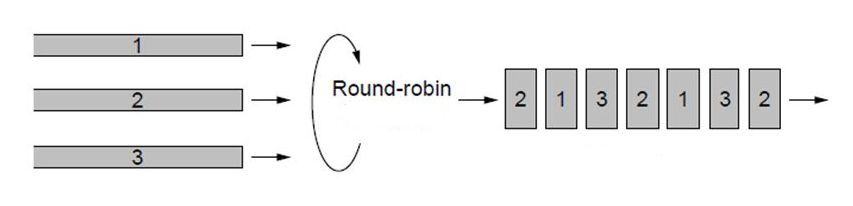
\includegraphics[width=0.8\textwidth]{round_robin.jpg}
            \caption{The Round Robin scheduler}
            \label{fig:RoundRobin}
        \end{figure}

    \subsubsection{First Come First Served}
        The project also implements the First Come First Served process
        scheduler -- in contrast to the Round Robin scheduler, this gives a
        process use of the CPU until it no longer needs it. While this seems
        less ``fair'' (precise scheduling criteria can be found at
        \cite[pg.~265]{DinosaurOS}), this scheduling policy may find use if it
        is vital that processes are executed in the order they are received.
        This algorithm is simple and provided largely to illustrate the use of
        compile-time options to configure the system, one of the key goals of
        the project.

    \subsubsection{Extension}
        With ease of extension a key consideration of this project, especially
        for a task such as process scheduling, care was taken in designing the
        interface for adding new scheduling algorithms. In particular, as it
        stands, all the code required for configuring the scheduling policy to
        use is contained in the file \code{sched.h} -- all that is required to
        add a policy to the system is to a) write the function that will be
        passing control to and taking control from the CPU, and b) add a case in
        the include guards to add this new scheduler as an option, so that the
        correct scheduler is used. A global function pointer, \code{void
        (*schedule)(void)}, taking no arguments and returning nothing, is used
        to set the scheduling policy of the system, and is set by testing which
        command-line options have been passed by the Makefile. The interface is
        covered more in depth in Section \ref{sec:Configuration}.

        Overall this interface works well -- it allows for the different
        schedulers to be switched between easily and with little effort. Its
        ease of extension could, however, face challenges as the policies the
        schedulers adopt become more complex. The scheduler the system uses is
        innately tied to influences how a process is represented in that system;
        for example, if one wanted to implement priority scheduling
        \cite[pg.~210]{DinosaurOS}, the structure \code{struct proc} would need
        to be extended to include how important it is that a given process is
        executed, with potentially a field to describe how this may change over
        time (aging). Therefore, changes will need to be made to at least the
        files \code{proc.h}, \code{sched.h}, and \code{sched.c}. This could
        eventually become cumbersome, and is not a consideration that the
        project takes in its current form. Furthermore, when using the First
        Come First Served scheduler, it does not disable the triggering of
        interrupts after a quantum has passed, but rather just ignores them.
        While this works, it is perhaps conceptually bad practise, and could
        lead to confusion, which this project aims to explicitly avoid. While
        there has not been the time or urgency to focus on this so far, it will
        certainly be a consideration in the future.

\subsection{Synchronisation}
    Since the project is a concurrent system, there is the possibility for race
    conditions -- the outcome of a computation being affected by the order in
    which processes access data. For this, we implement two forms of locks:
    spinlocks and semaphores. Both rely on the concept of an atomic operation,
    which is a computation that is performed with the guarantee of not being
    interrupted. For this purpose, ARM provides the \code{swp} instruction
    \cite{OnlineARMGuide}, essentially allowing us to ``acquire'' the lock first
    and then check that we have been successful, as opposed to the other way
    around. The implementation of a such an operation is given in Listing
    \ref{lst:Lock}.

    \lstset{language=c}
    \begin{lstlisting}[caption={Atomic lock
    operation},captionpos=b,label={lst:Lock}]
/* int try_lock(int *) */
try_lock:
    mov r1, #0
    swp r2, r1, [r0]
    mov r0, r2
    blx lr
    \end{lstlisting}

    We use this to implement the most basic form of synchronisation, the
    spinlock. This involves constantly trying to acquire the lock until it is
    successful. We initialise the lock value to 1, and the lock only
    successfully acquires it if it finds the result of \code{try\_lock()} is 1.

    More useful is a semaphore, and in particular the project implements the
    design outlined in \cite[pg.~265]{DinosaurOS}. To reduce the wastage of CPU
    cycles caused by busy-waiting that spinlocks entail, we instead maintain a
    list of processes that wish to acquire the semaphore: each process in this
    queue will be placed in the waiting state, meaning that the CPU scheduler
    can transfer control of the CPU to another process that is in the ready
    queue. This greatly increases CPU usage as control is always given to a
    process that can perform meaningful work with it, rather that simply waiting
    for the lock variable. Later, when a process releases the lock, it uses this
    wait queue to give the lock to the next process that was waiting for it.

    The implementation of this synchronisation interface takes inspiration from
    the POSIX mutex library \cite{POSIX_mutex}, albeit far more simplified,
    requiring only one single-parameter function call to initialise a given
    lock. When \code{mutex\_lock()} is called, a process tries acquire the lock
    and is either given the lock or placed on the wait queue, while
    \code{mutex\_unlock()} simply gives the lock to the next process in the
    queue.

\subsection{Configuration}
    \label{sec:Configuration}
    As mentioned, one of the key aims of the project was to present both an
    extensible and configurable operating system in order to demystify certain
    aspects about their development. While being clear to read and understand is
    useful, the ability to actively change key systems at compile-time provides
    a much more practical and hands-on opportunity to understand the key
    concepts that underpin the system. The main aspect to system configuration
    in this project is the use of Makefile directives, which provides an
    intuitive interface to quickly compile the system to make use of different
    approaches, and while not used extensively so far, it is an interface whose
    simplicity to extend to more options in the future is helpful.

    \subsubsection{Makefile}
        Compile-time configuration is performed by sending command-line
        directives to the Makefile. In particular, the project makes use of the
        \code{-D} flag to define certain variables within the source code. For
        example, when the target model was switched to the Pi 1 Model B+ from
        the Pi 2 Model B as a result of difficulties with the framebuffer, the
        code that dealt with shutting down three of the four cores was simply
        wrapped in C preprocessor \code{\#if defined} tests, meaning it would
        only get executed if it is explicitly specified that we are compiling
        for the Raspberry Pi 2 Model B. If not, it is assumed that we compile
        for the Raspberry Pi 1. This solution was particularly useful as it
        makes the codebase more portable to other models, without breaking its
        functionality on the current model and without requiring to delete the
        code entirely.

        Even more useful, considering the initial goals of the project, is the
        ability to load different process schedulers at compile-time. This is
        achieved in much the same way as how the model of Raspberry Pi is
        targeted -- we simply wrap the blocks of code corresponding to the
        different options available in preprocessor expressions, and set the
        \code{void (*schedule)(void)} function accordingly. Listing
        \ref{lst:Make_example} gives an example issue of the \code{make} command
        with command-line directives sent to the preprocessor, and shows which
        directives they define. Listing \ref{lst:schedulefn} shows how this
        interface is used to determine which scheduling function to compile.
        Just as the model requires a default value, we assume the default
        scheduler to use is the Round Robin algorithm.

        \begin{lstlisting}[caption={An example \code{make} command, and the
        directives it defines},captionpos=b,label={lst:Make_example}]
make model=1 sched=robin
DIRECTIVES = -DRPIBPLUS -DSCHED_ROUNDROBIN
        \end{lstlisting}

        \begin{lstlisting}[caption={Configuring the scheduling algorithm at
        compile-time},captionpos=b,label={lst:schedulefn}]
#if defined ( SCHED_FCFS )
    schedule = sched_fcfs;
    strcpy(sch_str, "FCFS");
#elif defined ( SCHED_ROUNDROBIN )
    schedule = sched_round_robin;
    strcpy(sch_str, "Round Robin");
#else
    schedule = sched_round_robin;
    strcpy(sch_str, "Round Robin");
#endif
        \end{lstlisting}

\subsection{Ongoing development}
    The project, while functional in what it implements, is not in an entirely
    complete state. Two systems in particular have been developed to an extent,
    but work is required to integrate them fully into the operating system --
    these are the tasks of inter-process communication and user interaction via
    a keyboard.

    \subsubsection{Inter-process Communication}
        The project implements a functional but rudimentary form of the
        shared-memory model of inter-process communication. This involves
        declaring a new structure, \code{struct shm\_section}, which contains
        fields describing its address in memory, an identifying name, and a
        character array to storo data written to it. We create a new shared
        memory section by allocating a new page, with the \code{shared} bit set.
        Another process may then use the data in this page with calls to
        \code{shm\_read()} and \code{shm\_write()}, which simply perform MMIO
        with extra checks for validity of access.

    \subsubsection{Keyboard input}
        Keyboard input is generally done via USB keyboard on the Raspberry Pi,
        although we may use the UART peripheral to receive input from a keyboard
        using a USB-to-TTL adapter. Since the USB standard is designed to
        accommodate a wide variety of hardware devices, with USB ports
        themselves containing only 4 pins, this means much of the functionality
        must be implemented in hardware. However, the time frame of the project
        did not allow for such a task as implementing a USB keyboard driver from
        scratch. Instead, it was opted to use a static library to provide the
        functionality of user interaction. In particular, Rene Stange provides
        such a driver \cite{USPi}, whose compilation may be tweaked depending on
        the target environment. This is then archived into a static library,
        whose functions may be accessed by supplying it to the linker at
        compile-time. In the case of this project, this is done by specifying
        \code{-luspi} as a linker flag in the Makefile. However, this solution
        still too remains in the process of being developed to be entirely
        functional.
